% mnras_template.tex 
%
% LaTeX template for creating an MNRAS paper
%
% v3.0 released 14 May 2015
% (version numbers match those of mnras.cls)
%
% Copyright (C) Royal Astronomical Society 2015
% Authors:
% Keith T. Smith (Royal Astronomical Society)

% Change log
%
% v3.0 May 2015
%    Renamed to match the new package name
%    Version number matches mnras.cls
%    A few minor tweaks to wording
% v1.0 September 2013
%    Beta testing only - never publicly released
%    First version: a simple (ish) template for creating an MNRAS paper

%%%%%%%%%%%%%%%%%%%%%%%%%%%%%%%%%%%%%%%%%%%%%%%%%%
% Basic setup. Most papers should leave these options alone.
\documentclass[fleqn,usenatbib]{mnras}

% MNRAS is set in Times font. If you don't have this installed (most LaTeX
% installations will be fine) or prefer the old Computer Modern fonts, comment
% out the following line
\usepackage{newtxtext,newtxmath}
% Depending on your LaTeX fonts installation, you might get better results with one of these:
%\usepackage{mathptmx}
%\usepackage{txfonts}

% Use vector fonts, so it zooms properly in on-screen viewing software
% Don't change these lines unless you know what you are doing
\usepackage[T1]{fontenc}

% Allow "Thomas van Noord" and "Simon de Laguarde" and alike to be sorted by "N" and "L" etc. in the bibliography.
% Write the name in the bibliography as "\VAN{Noord}{Van}{van} Noord, Thomas"
\DeclareRobustCommand{\VAN}[3]{#2}
\let\VANthebibliography\thebibliography
\def\thebibliography{\DeclareRobustCommand{\VAN}[3]{##3}\VANthebibliography}


%%%%% AUTHORS - PLACE YOUR OWN PACKAGES HERE %%%%%

% Only include extra packages if you really need them. Common packages are:
\usepackage{graphicx}	% Including figure files
\usepackage{amsmath}	% Advanced maths commands
\usepackage{amssymb}	% Extra maths symbols

%%%%%%%%%%%%%%%%%%%%%%%%%%%%%%%%%%%%%%%%%%%%%%%%%%

%%%%% AUTHORS - PLACE YOUR OWN COMMANDS HERE %%%%%

% Please keep new commands to a minimum, and use \newcommand not \def to avoid
% overwriting existing commands. Example:
%\newcommand{\pcm}{\,cm$^{-2}$}	% per cm-squared

%%%%%%%%%%%%%%%%%%%%%%%%%%%%%%%%%%%%%%%%%%%%%%%%%%

%%%%%%%%%%%%%%%%%%% TITLE PAGE %%%%%%%%%%%%%%%%%%%

% Title of the paper, and the short title which is used in the headers.
% Keep the title short and informative.
\title[Short title, max. 45 characters]{MNRAS \LaTeXe\ template -- title goes here}

% The list of authors, and the short list which is used in the headers.
% If you need two or more lines of authors, add an extra line using \newauthor
\author[D. Neill et al.]{
Duncan Neill,$^{1}$\thanks{E-mail: dn431@bath.ac.uk}
William Newton,$^{2}$
David Tsang$^{1}$
\\
% List of institutions
$^{1}$Department of Physics, University of Bath, Claverton Down, Bath, BA1 1AL\\
$^{2}$Department of Physics and Astronomy, Texas A\&M University-Commerce, Commerce, TX, 75429-3011
}

% These dates will be filled out by the publisher
\date{Accepted XXX. Received YYY; in original form ZZZ}

% Enter the current year, for the copyright statements etc.
\pubyear{2015}

% Don't change these lines
\begin{document}
\label{firstpage}
\pagerange{\pageref{firstpage}--\pageref{lastpage}}
\maketitle

% Abstract of the paper
\begin{abstract}
We do physics and calculate stuff. 
Such Physics. Many maths. Wow.
\end{abstract}

% Select between one and six entries from the list of approved keywords.
% Don't make up new ones.
\begin{keywords}
keyword1 -- keyword2 -- keyword3
\end{keywords}

%%%%%%%%%%%%%%%%%%%%%%%%%%%%%%%%%%%%%%%%%%%%%%%%%%

%%%%%%%%%%%%%%%%% BODY OF PAPER %%%%%%%%%%%%%%%%%%

% \section{Introduction}

% This is a simple template for authors to write new MNRAS papers.
% See \texttt{mnras\_sample.tex} for a more complex example, and \texttt{mnras\_guide.tex}
% for a full user guide.

% All papers should start with an Introduction section, which sets the work
% in context, cites relevant earlier studies in the field by \citet{Fournier1901},
% and describes the problem the authors aim to solve \citep[e.g.][]{vanDijk1902}.
% Multiple citations can be joined in a simple way like \citet{deLaguarde1903, delaGuarde1904}.

% \section{Methods, Observations, Simulations etc.}

% Normally the next section describes the techniques the authors used.
% It is frequently split into subsections, such as Section~\ref{sec:maths} below.

% \subsection{Maths}
% \label{sec:maths} % used for referring to this section from elsewhere

% Simple mathematics can be inserted into the flow of the text e.g. $2\times3=6$
% or $v=220$\,km\,s$^{-1}$, but more complicated expressions should be entered
% as a numbered equation:

% \begin{align}
%     x=\frac{-b\pm\sqrt{b^2-4ac}}{2a}.
% 	\label{eq:quadratic}
% \end{align}

% Refer back to them as e.g. equation~(\ref{eq:quadratic}).

% \subsection{Figures and tables}

% Figures and tables should be placed at logical positions in the text. Don't
% worry about the exact layout, which will be handled by the publishers.

% Figures are referred to as e.g. Fig.~\ref{fig:example_figure}, and tables as
% e.g. Table~\ref{tab:example_table}.

% % Example figure
% \begin{figure}
% 	% To include a figure from a file named example.*
% 	% Allowable file formats are eps or ps if compiling using latex
% 	% or pdf, png, jpg if compiling using pdflatex
% 	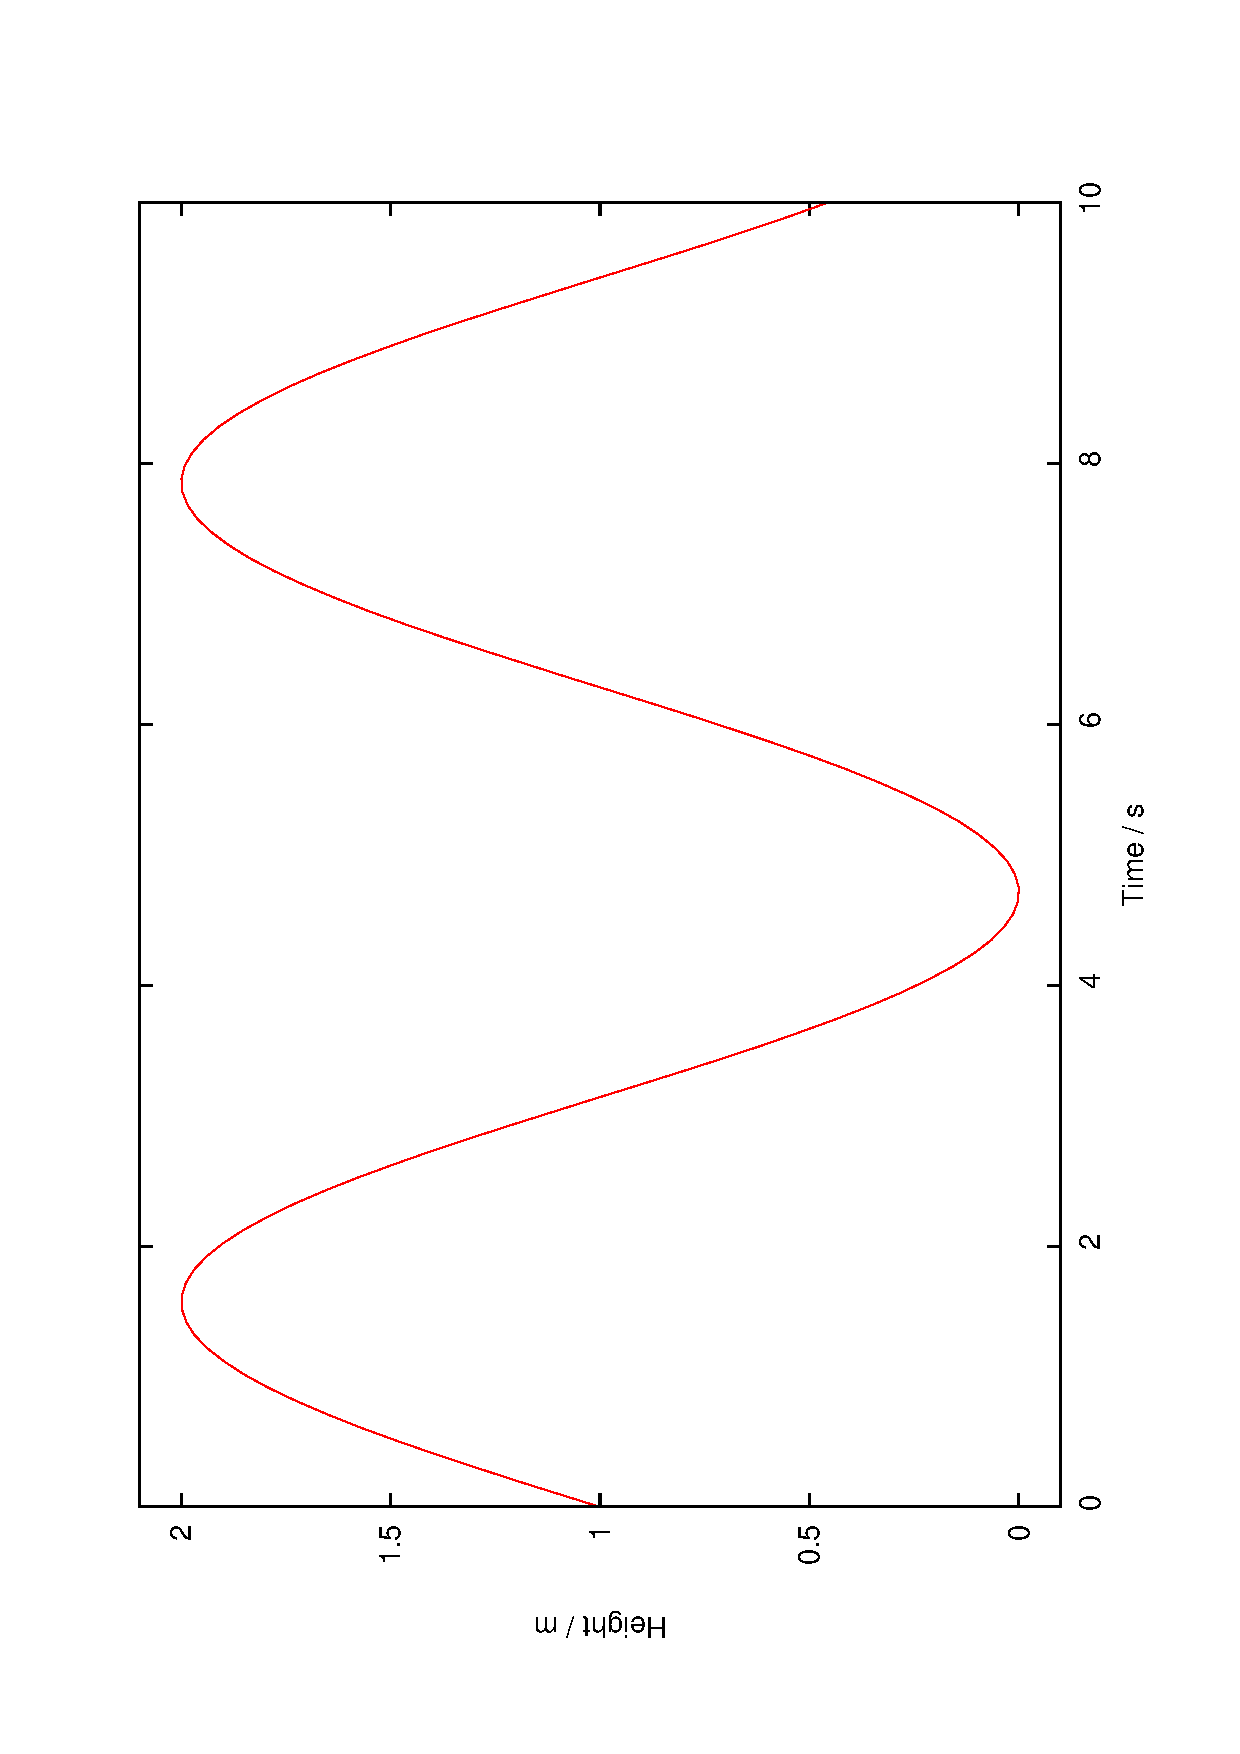
\includegraphics[width=\columnwidth]{example}
%     \caption{This is an example figure. Captions appear below each figure.
% 	Give enough detail for the reader to understand what they're looking at,
% 	but leave detailed discussion to the main body of the text.}
%     \label{fig:example_figure}
% \end{figure}

% % Example table
% \begin{table}
% 	\centering
% 	\caption{This is an example table. Captions appear above each table.
% 	Remember to define the quantities, symbols and units used.}
% 	\label{tab:example_table}
% 	\begin{tabular}{lccr} % four columns, alignment for each
% 		\hline
% 		A & B & C & D\\
% 		\hline
% 		1 & 2 & 3 & 4\\
% 		2 & 4 & 6 & 8\\
% 		3 & 5 & 7 & 9\\
% 		\hline
% 	\end{tabular}
% \end{table}


% \section{Conclusions}

% The last numbered section should briefly summarise what has been done, and describe
% the final conclusions which the authors draw from their work.

% \section*{Acknowledgements}

% The Acknowledgements section is not numbered. Here you can thank helpful
% colleagues, acknowledge funding agencies, telescopes and facilities used etc.
% Try to keep it short.

% %%%%%%%%%%%%%%%%%%%%%%%%%%%%%%%%%%%%%%%%%%%%%%%%%%
% \section*{Data Availability}

 
% The inclusion of a Data Availability Statement is a requirement for articles published in MNRAS. Data Availability Statements provide a standardised format for readers to understand the availability of data underlying the research results described in the article. The statement may refer to original data generated in the course of the study or to third-party data analysed in the article. The statement should describe and provide means of access, where possible, by linking to the data or providing the required accession numbers for the relevant databases or DOIs.

\section{Introduction}
\hspace{\parindent}Neutron stars consist of extremely dense matter, the study of which is important for our understanding of nuclear physics. To study the internal structure of these stars and the nuclear physics that determines it, we must find ways to probe them using observational phenomena. Short gamma-ray bursts (sGRBs)~\cite{d2015short} are one such phenomena that, while their origins are uncertain, are likely originate from the merging of binary neutron stars. Around 10\% of sGRBs are preceded by a 'precursor' flare~\cite{troja2010precursors}. These precursor flares can be identified as a lower, separate peak in the gamma-ray count a short time ($\sim 0.1-1.0$ s) before the main peak~\cite{zhong2019precursors}. 
%mention possible causes of precursors (here or later?)

\hspace{\parindent}In the last few years multi-messenger observations of neutron star mergers have provided insight into the origin of sGRBs. In particular, the detection of the gravitational wave signals GW170817~\cite{abbott2017merger} and GW190425~\cite{abbott2020gw190425} that are thought to originate from mergers has provided a new angle from which to investigate neutron stars. Here, we use the frequency of gravitational waves to investigate the possibility of a relationship between precursor flares and the modes of oscillation within a neutron star.

\hspace{\parindent}Within a star the bulk motion of matter can be depicted as a combination of an infinite set of oscillation modes~\cite{smeyers2011linear}, each of which obeys the boundary conditions for the displacement of matter at the surface and core of the star. Each mode can be defined by the frequency at which it oscillates and the displacement of matter it causes throughout the star. These oscillations can be driven by external gravitational fields, such as that of a binary partner. They are strongly dependant on the internal structure of the star, with different modes being dependant on different properties, such as pressure or shear forces.








\subsection{Resonant Shattering Flares}
\hspace{\parindent}During the in-spiral of binary neutron stars, the oscillation modes can become excited by the tidal forces from the binary partner. Each oscillation mode overlaps with the tidal field to a different degree, which determines that amount of energy deposited in that specific mode. As the stars' orbits get smaller, the frequency of the orbit (and hence the gravitational wave frequency) increases. When the orbital frequency matches a mode's frequency it may become resonantly excited, causing the oscillations to rapidly grow in magnitude~\cite{tsang2012resonant}~\cite{tsang2013shattering}.

\hspace{\parindent}The theory of resonant shattering flares is that if the overlap between the tidal field and an oscillation mode is great enough, the resonant excitation of that mode may cause the neutron star crust to become deformed~\cite{troja2010precursors}. If this deformation becomes large enough the strain in the crust may exceed its limit, causing it to fracture which depositing seismic energy in the crust. If enough energy is deposited in the crust it could shatter, creating high frequency oscillations that couple to the magnetic field to release a precursor flare shortly before the main sGRB.%explain RSF process better, explain (why)/(what is) the interface mode

\hspace{\parindent}Using multi-messenger observations of neutron star mergers, it is possible that the gravitational wave frequency at which a precursor flare occurs could be found. In order for a resonant shattering flare to occur, the frequency of the gravitational waves (i.e. the orbital frequency) must be similar to the frequency of the crust-core interface mode. Therefore, by calculating the frequency of the interface mode using a variety of nuclear models the nuclear parameters could be restricted to those that result in a mode frequency that closely matches the observed gravitational wave frequency during the precursor flare.



\subsection{Nuclear Symmetry Energy and Neutron Star Structure}
\hspace{\parindent}The oscillation frequencies of the modes are dependant on the neutron star equation of state (EoS), the relationship between the energy density and pressure inside the star. At low densities the EoS is well known. %from what? (references)
However, at the extreme densities found in neutron stars the EoS is poorly understood and therefore we must rely on nuclear models. These models can be parameterised by various nuclear properties in order to reproduce physical results. One such set of parameters are the nuclear symmetry energy parameters. The nuclear symmetry energy is the energy required to convert a proton into a neutron (or vice-versa) in symmetric matter. At nuclear saturation density (the density of nucleons in a nucleus) the first three symmetry energy parameters are: the symmetry energy
\begin{align}
J=E_{\rm sym}(n_0),    
\label{eq:sym_J}
\end{align}
\noindent its first derivative 
\begin{align}
L=\frac{\partial E_{\rm sym}(n_b)}{\partial \chi}\biggr\rvert_{n_b=n_0},  
\label{eq:sym_L}
\end{align}
\noindent and its second derivative
\begin{align}
K_{\rm sym}=\frac{\partial^2 E_{\rm sym}(n_b)}{\partial \chi^2}\biggr\rvert_{n_b=n_0},
\label{eq:sym_K}
\end{align}
\noindent where $\chi=\frac{n_b-n_0}{3n_0}$.

\hspace{\parindent}To investigate the nuclear symmetry energy parameters we generated a set of EoSs parameterised by a range of values for $J$ ,$L$ and $K_{\rm sym}$. By calculating the mode frequencies for these EoSs we are able to find the relationship between the symmetry energy parameters and the gravitational wave frequency at which a RSF occurs.
%J,L,K_sym used to parameterise the EoS -> structure determined by EoS -> mode frequency dependant on structure, so frequency at which RSF occurs is dependant on symmetry energy parameters

\section{Parameterised Neutron Star Equation of State and Composition}


\section{Calculation of the Normal Modes}
\hspace{\parindent}Each mode of oscillation gives a different profile of the radial and transverse displacements. To calculate this, as well as the frequency the modes oscillate at, we perturb the equations defining the equilibrium state of neutron star matter.

\hspace{\parindent}The neutron stars involved in mergers are old and therefore will have cooled to low temperatures, and so we adopt the zero temperature limit. We also assume that the periods of the modes of interest are significantly lower that the beta equilibrium timescale. Finally, we ignore terms that are non-linear in perturbations, as the perturbations are small and therefore non-linear terms are negligible.




% ASSUME ZERO SPIN -> HENCE WHY IN RESULTS SECTION RANGE IN MASS (1.17-1.36, 1.36-1.60) IS THE MASS MEASUREMENTS ASSUMING LOW NS SPIN.
%Eulerian vs Lagrangian perturbations
\subsection{Linear Perturbation Equations}
\hspace{\parindent}Following the methodology of~\cite{mcdermott1988nonradial}, the equations governing the displacement caused by the modes of oscillation can be derived from the equations for mass continuity, momentum conservation, and Poisson's equation:
\begin{align}
\frac{\partial\rho}{\partial t}+\nabla\cdot(\rho v)=0,
\label{eq:continuity_eqn}
\end{align}
\begin{align}
\frac{\partial v}{\partial t}=(v\cdot \nabla)v=\frac{1}{\rho}\nabla\cdot\sigma-\nabla\Phi,
\label{eq:momentum_eqn}
\end{align}
\begin{align}
\nabla^2\Phi=4\pi G\rho,
\label{eq:Poisson_eqn}
\end{align}
\noindent where $\rho$ is the energy density, $v$ is the velocity of the matter, $\sigma$ is the stress tensor, and $\Phi$ is the gravitational potential. By adding a small perturbation to each of the quantities in these equations (ie: $\rho\rightarrow\rho+\delta\rho$), and ignoring terms that are non-linear in perturbations, these three equations can be used to obtain the wave equation
\begin{eqnarray}\nonumber
\sigma^2 u&=& -\nabla\left(\frac{\Gamma_1 p}{\rho}\nabla\cdot u\right)-\nabla\left(\frac{1}{\rho}u\cdot\nabla p\right)-\hat{r}A\frac{\Gamma_1 p}{\rho}\nabla\cdot u+\nabla\Phi '\\\nonumber
&&+\frac{1}{\rho}\biggr(\nabla\left(\frac{2}{3}\mu\nabla\cdot u\right)-\left(\nabla\mu\cdot\nabla\right)u-\nabla\left(u\cdot\nabla\mu\right)\\
&&+\left(u\cdot\nabla\right)\nabla\mu-\mu\left(\nabla^2 u+\nabla\left(\nabla\cdot u\right)\right)\biggr),
\label{eq:wave_eqn}
\end{eqnarray}
where $u(x,t)$ is the Lagrangian displacement. The time dependence of the perturbed quantities was assumed to be of the form $e^{i\sigma t}$, with $\sigma$ being the frequency of the mode's oscillations. This can be used to separate the time and position dependencies of the Lagrangian displacement to get $u(x,t)=\xi(x)e^{i\sigma t}$. In spherical coordinates this can be further separated into radial and transverse components:
\begin{align}\nonumber
\xi_r=U(r)Y_{lm},\;\;\;\xi_{\theta}=V(r)\frac{\partial Y_{lm}}{\partial\theta},
\end{align}
\begin{align}
\xi_{\phi}=\frac{V(r)}{sin(\theta)}\frac{\partial Y_{lm}}{\partial\phi},\;\;\;\Phi '=\hat{\Phi}'(r)Y_{lm},
\label{eq:xi_seperation}
\end{align}
\noindent with $U(r)$ being the radial displacement, $V(r)$ being the transverse displacement, and $Y_{lm}$ being the spherical harmonics.

\hspace{\parindent}By using the separation of variables given in equation \ref{eq:xi_seperation}, and using $u(x,t)=\xi(x)e^{i\sigma t}$ to remove the time dependence, equation \ref{eq:wave_eqn} becomes a set of 5 equations:
\begin{eqnarray}\nonumber
\rho\sigma^2U&=& \rho\frac{d\hat{\chi}}{dr}-A\Gamma_1 p\hat{\alpha}-\frac{d}{dr}\left(\frac{1}{3}\mu\hat{\alpha}\right)+\frac{d\mu}{dr}\left(\hat{\alpha}-2\frac{dU}{dr}\right)\\
&&-\mu\left(\frac{1}{r^2}\frac{d}{dr}\left( r^2\frac{dU}{dr}\right)-\frac{l(l+1)}{r^2}U+\frac{2l(l+1)}{r^2}V\right),
\label{eq:Ueqn}
\end{eqnarray}
\begin{eqnarray}\nonumber
\rho\sigma^2V&=&\rho\frac{\hat{\chi}}{r}-\frac{1}{3}\frac{\mu\hat{\alpha}}{r}-\frac{d\mu}{dr}\left(\frac{dV}{dr}-\frac{V}{r}+\frac{U}{r}\right)\\
&&-\mu\left(\frac{1}{r^2}\frac{d}{dr}\left(r^2\frac{dV}{dr}\right)-\frac{l(l+1)}{r^2}V+\frac{2}{r^2}U\right),
\label{eq:Veqn}
\end{eqnarray}
\begin{align}
\frac{1}{r^2}\frac{d}{dr}\left(r^2\frac{d\hat{\Phi}'}{dr}\right)-\frac{l(l+1)}{r^2}\hat{\Phi}'=4\pi G\left(U\frac{d\rho}{dr}+\hat{\alpha}\rho\right),
\label{eq:Phihat_eqn}
\end{align}
\noindent where:
\begin{align}
\hat{\alpha}=\frac{1}{r^2}\frac{d}{dr}(r^2U)-\frac{l(l+1)}{r}V,
\label{eq:alphahat}
\end{align}
\begin{align}
\hat{\chi}=-\frac{\Gamma_1p}{\rho}\hat{\alpha}-\frac{1}{\rho}\frac{\partial p}{\partial r}U+\hat{\Phi}'.
\label{eq:chihat}
\end{align}
\noindent These equations are simplified by taking the Cowling approximation (\cite{cowling1941non}). This approximation states that, since the mass of a star is concentrated in its centre, the displacement of matter away from the core does not significantly alter the gravitational potential. Therefore we use ($\Phi '\approx 0$).



\hspace{\parindent}For the fluid core of a neutron star, equations \ref{eq:Ueqn}-\ref{eq:chihat} are further simplified because in a fluid the shear modulus ($\mu$) must be zero. By using $\mu=0$, and be rewriting $U$ and $V$ as the dimensionless variables
\begin{align}
y_1=\frac{U}{r},\;\;\;\;y_2=\frac{\sigma^2V}{g}
\label{eq:y1y2}
\end{align}
\noindent (where $g=\frac{1}{\rho}\frac{dP}{dr}$), equations \ref{eq:Ueqn}-\ref{eq:chihat} can be rewritten as a pair of coupled differential equations:
\begin{align}
\left(1+\tilde{V}\right)\frac{dy_1}{dx}=\left(\frac{\tilde{V}}{\Gamma_1}-3\right)y_1+\left(\frac{l(l+1)}{c_1\Omega^2}-\frac{\tilde{V}}{\Gamma_1}\right)y_2,
\label{eq:McDy1}
\end{align}
\begin{align}
\left(1+\tilde{V}\right)\frac{dy_2}{dx}=\left(c_1\Omega^2+Ar\right)y_1+\left(1-\tilde{U}-Ar\right)y_2,
\label{eq:McDy2}
\end{align}
\noindent where the equilibrium properties of the star are: 
\begin{align}\nonumber
\tilde{U}=\frac{d\:ln\left(M_r\right)}{d\:ln\left(r\right)}=4\pi r^2\rho\frac{r}{M_r},\;\;\;c_1=\left(\frac{r}{R_*}\right)^3\frac{M_*}{M_r},\;\;\;\Omega^2=\frac{\sigma^2R_*^3}{GM_*},
\label{eq:eqbm_properties1}
\end{align}
\begin{align}\nonumber
\tilde{V}=-\frac{d\:ln\left(P\right)}{d\:ln\left(r\right)}=-\frac{G\rho M_r}{rP}\left(1+\frac{P}{\rho c^2}\right)\left(1+\frac{4\pi r^3 P}{M_r c^2}\right)\left(1-\frac{2GM_r}{rc^2}\right)^{-1},
\label{eq:eqbm_properties2}
\end{align}
\begin{align}
A=\frac{1}{\rho}\frac{d\rho}{dr}-\frac{1}{\Gamma_1P}\frac{dP}{dr}
\label{eq:schwartz_descrim}
\end{align}
\noindent is the Schwarzschild discriminant, and
\begin{align}
\Gamma_1=\left(\frac{\partial\:ln(P)}{\partial\:ln(\rho)}\right)_s
\label{eq:adiabatic_index}
\end{align}
\noindent is the adiabatic index when the composition of the star is frozen.



\hspace{\parindent}For the solid crust the shear modulus is not zero, and therefore we obtain a set of four coupled differential equations:
\begin{align}
\left(1+\tilde{V}\right)\frac{dz_1}{dx}=-\left(1+2\frac{\alpha_2}{\alpha_3}\right)z_1+\frac{1}{\alpha_3}z_2+l\left(l+1\right)\frac{\alpha_2}{\alpha_3}z_3,
\label{eq:z1dr}
\end{align}
\begin{eqnarray}\nonumber
\left(1+\tilde{V}\right)\frac{dz_2}{dx}&=&\left(-\tilde{V}c_1\Omega^2-4\tilde{V}+\tilde{U}\tilde{V}+12\Gamma_1\frac{\alpha_1}{\alpha_3}\right)z_1\\\nonumber
&&+\left(\tilde{V}-4\frac{\alpha_1}{\alpha_3}\right)z_2+l\left(l+1\right)\left(\tilde{V}-6\Gamma_1\frac{\alpha_1}{\alpha_3}\right)z_3\\
&&+l\left(l+1\right)z_4,
\label{eq:z2dr}
\end{eqnarray}
\begin{align}
\left(1+\tilde{V}\right)\frac{dz_3}{dx}=-z_1+\frac{1}{\alpha_1}z_4,
\label{eq:z3dr}
\end{align}
\begin{eqnarray}\nonumber
\left(1+\tilde{V}\right)\frac{dz_4}{dx}&=& \biggr(-\tilde{V}c_1\Omega^2+\frac{2}{\alpha_3}\biggr((2l(l+1)-1)\alpha_1\alpha_2\\\nonumber
&&+2(l(l+1)-1)\alpha_1^2\biggr)\biggr)z_3\\
&&+\left(\tilde{V}-6\Gamma_1\frac{\alpha_1}{\alpha_3}\right)z_1-\frac{\alpha_2}{\alpha_3}z_2+(\tilde{V}-3)z_4,
\label{eq:z4dr}
\end{eqnarray}
\noindent where $\alpha_1=\frac{\mu}{\rho}$, $\alpha_2=\Gamma_1-\frac{2}{3}\frac{\mu}{\rho}$, $\alpha_2=\Gamma_1+\frac{4}{3}\frac{\mu}{\rho}$, and the dimensionless variables are 
\begin{eqnarray}
&z_1=\frac{U}{r},&z_2=\frac{1}{\rho}\left((\Gamma_1p-\frac{2}{3}\mu)\hat{\alpha}+2\mu\frac{dU}{dr}\right),\\
&z_3=\frac{V}{r},&z_4=\frac{\mu}{p}\left(\frac{dV}{dr}-\frac{V}{r}+\frac{U}{r}\right).
\label{eq:z1z2z3z4}
\end{eqnarray}
\noindent $z_1$ is the radial displacement, $z_2$ is proportional to the radial traction, $z_3$ is the transverse displacement, $z_1$ is proportional to the transverse traction.



\hspace{\parindent}At the boundaries between the crust and the core, and the ocean and the crust, there are three jump conditions that must be satisfied:
\begin{align}
z_1=y_1,
\label{eq:jump1}
\end{align}
\begin{align}
z_2=\tilde{V}(y_1-y_2),
\label{eq:jump2}
\end{align}
\begin{align}
z_4=0.
\label{eq:jump3}
\end{align}
\noindent The first two of these conditions can be combined to obtain $\frac{z_2}{z_1}=\tilde{V}\left(1-\frac{y_2}{y_1}\right)$, resulting in two conditions and two eigenvalues, $\Omega$ and $z_3(R_*)$. 



\hspace{\parindent}For any mode the boundary conditions at the centre and surface of the star must be obeyed. The condition at the centre follows from the requirement that $y_1$ and $y_2$ be regular at $r=0$:
\begin{align}
\frac{c_1\Omega^2}{l}y_1-y_2=0.
\label{eq:core_condition}
\end{align}
\noindent The condition at the surface is based on the requirement that the Lagrangian pressure perturbation goes to zero at $r=R_*$ :
\begin{align}
\left(\tilde{V}-c_1\Omega^2-4+\tilde{U}\right)y_1+\left(\frac{l(l+1)}{c_1\Omega^2}-\tilde{V}\right)y_2=0,
\label{eq:surface_condition}
\end{align}
\noindent However, this boundary condition is for a fluid surface ocean. The ocean is negligible for the interface modes, and so we skip directly to the crust. Therefore the surface boundary condition must be combined with the jump conditions (equations \ref{eq:jump1}-\ref{eq:jump3}) to rewrite it as
\begin{align}
z_2=\tilde{V}\left(\frac{\tilde{V}-c_1\Omega^2-4+\tilde{U}}{\frac{l(l+1)}{c_1\Omega^2}-\tilde{V}}+1\right)z_1,
\label{eq:surface_boundary_modified_1}
\end{align}
\begin{align}
z_4=0.
\label{eq:surface_boundary_modified_2}
\end{align}



\hspace{\parindent}By using trial values for the eigenvalues and calculating the error in the two jump conditions, the modes can be found as the places where both conditions are satisfied. Figure \ref{fig:trace_minima} shows the locations of the zeros in the error of the conditions.

\begin{figure}
\centering
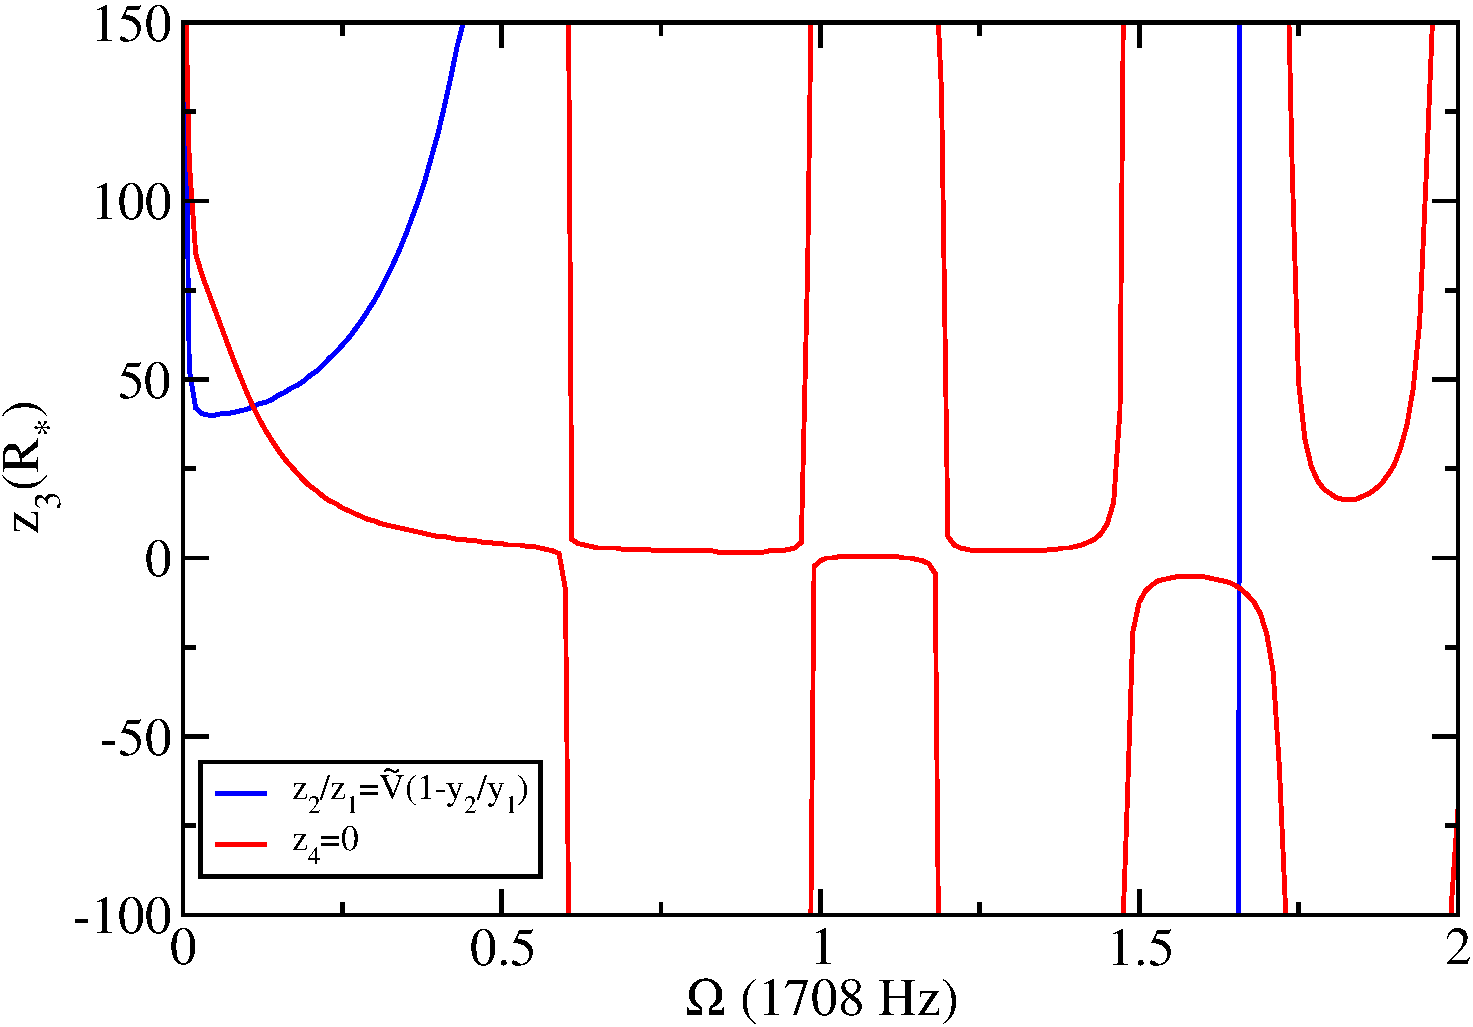
\includegraphics[width=0.45\textwidth,angle=0]{minima_new}
\caption{The minima of the error in the jump conditions at the crust-core boundary, showing the location of two modes for the sly4 EoS.}
\label{fig:trace_minima}
\end{figure}








\subsection{The Crust-Core Interface Mode}
\hspace{\parindent}For a neutron star with a fluid core and a solid crust, we are able to obtain the interface (i) mode. This mode, as shown in figure \ref{fig:imode_sly4}, has the radial displacement peaking at the crust-core boundary and is strongly dependant on the shear modulus of the crust, particularly at the base of the crust. It has a strong overlap with the tidal field, making it a good candidate for the source of RSFs as less time will be needed at resonance for it to reach the elastic limit for the crust to begin to fracture. For the sly4 EoS, its eigenvalues are $\Omega=0.1104$ and $z_3(R_*)=42.39$ (as can be seen in figure \ref{fig:trace_minima}), giving the mode a frequency of $188.5$ Hz. The transverse displacement in the core is small, while in the crust it discontinuously jumps to become large.

\begin{figure}
\centering
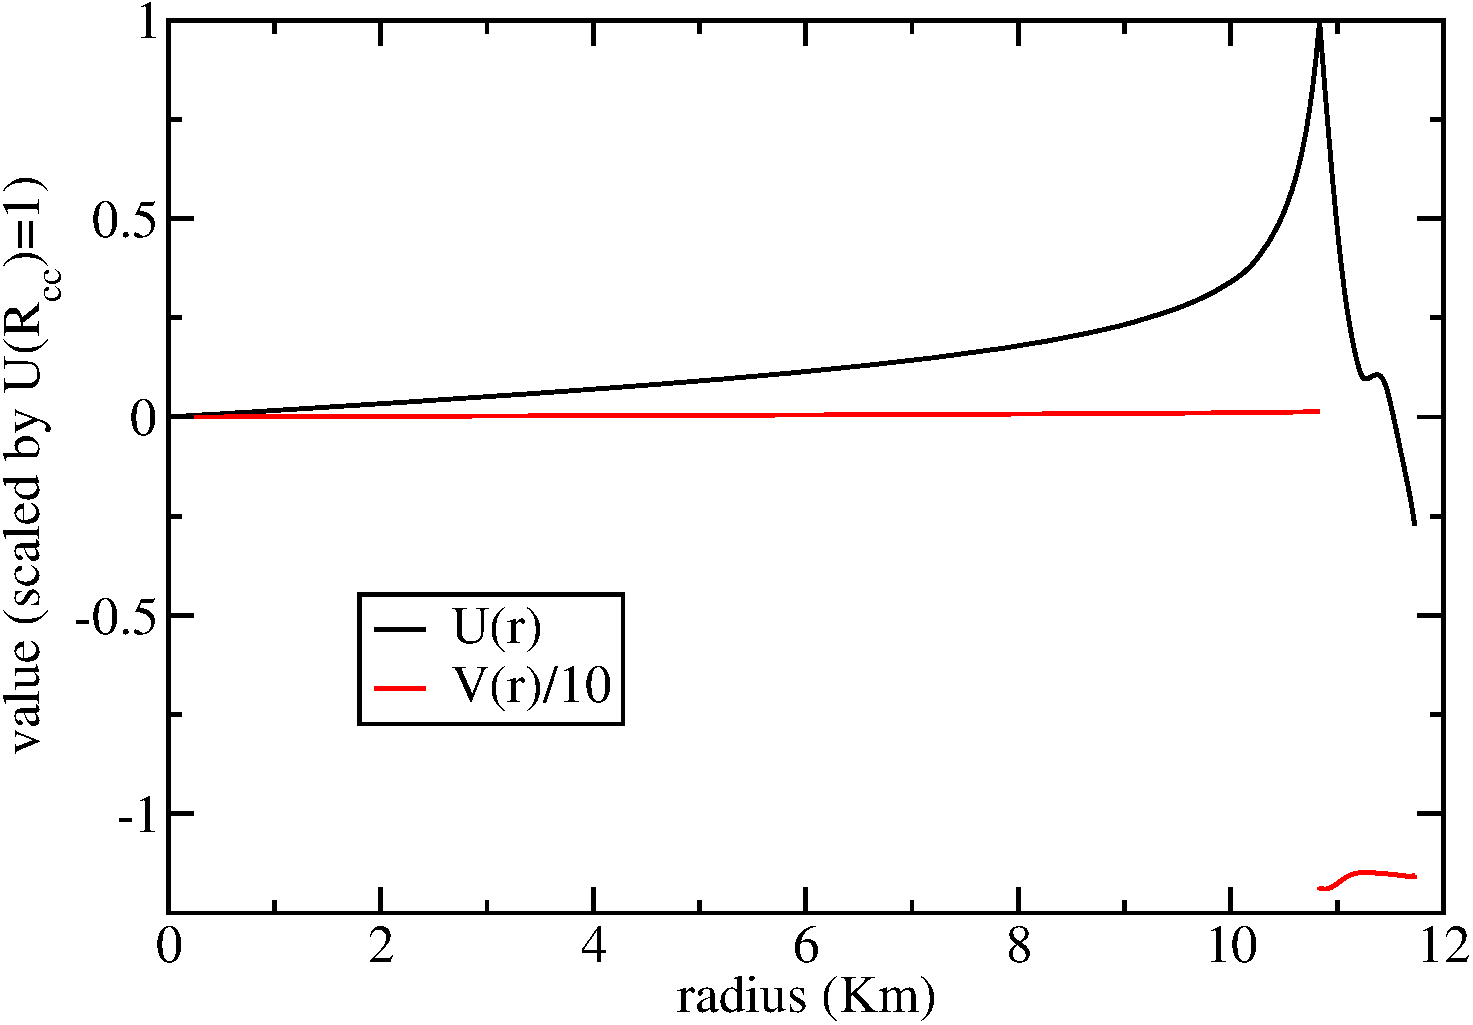
\includegraphics[width=0.45\textwidth,angle=0]{sly4_imode}
\caption{The 2i mode for the sly4 equation of state. $V(r)$ has been reduced by an order of magnitude so that it can be plotted alongside $U(r)$.}
\label{fig:imode_sly4}
\end{figure}

\hspace{\parindent}The i-mode has a strong dependence on the shear modulus in the crust, and more specifically at the crust-core transition. We investigate this dependence by considering a shear modulus scaled by 
\begin{align}
\tilde{\mu} = B \mu 
\end{align}

\begin{align}
\mu=\frac{A}{1+B\left(\frac{100}{\Gamma}\right)^2}\frac{n_i\left(Ze\right)^2}{a},
\label{eq:varymu}
\end{align}
\noindent where:
\begin{align}
a=\left(\frac{3}{4\pi n_i}\right)^{\frac{1}{3}},
\label{eq:mu1991a}
\end{align}
\begin{align}
\Gamma=\frac{\left(Ze\right)^2}{ak_bT}.
\label{eq:mu1991gamma}
\end{align}
\noindent This is the same as the formula given by Strohmayer in~\cite{strohmayer1991shear} when $A=0.1194$ and $B=1.781$. The constant $A$ scales the shear modulus, while the constant $B$ determines the dependence on $\Gamma$. These constants were varied to determine their impact on the i-mode. However, $\Gamma$ increases in the crust to quickly become large enough that $1>>\left(\frac{100}{\Gamma}\right)^2$, and therefore $B$ must be very large in order to cause any significant change in the shear modulus. Because of this only the results for varying $A$ are shown in figure \ref{fig:mu_A}. Modifying the shear modulus in this way is very artificial due to the shear modulus being strongly linked to the equilibrium properties of the star. Therefore, only changing the shear modulus should be seen as a rough guide to its impact on the frequency.

\begin{figure}
\centering
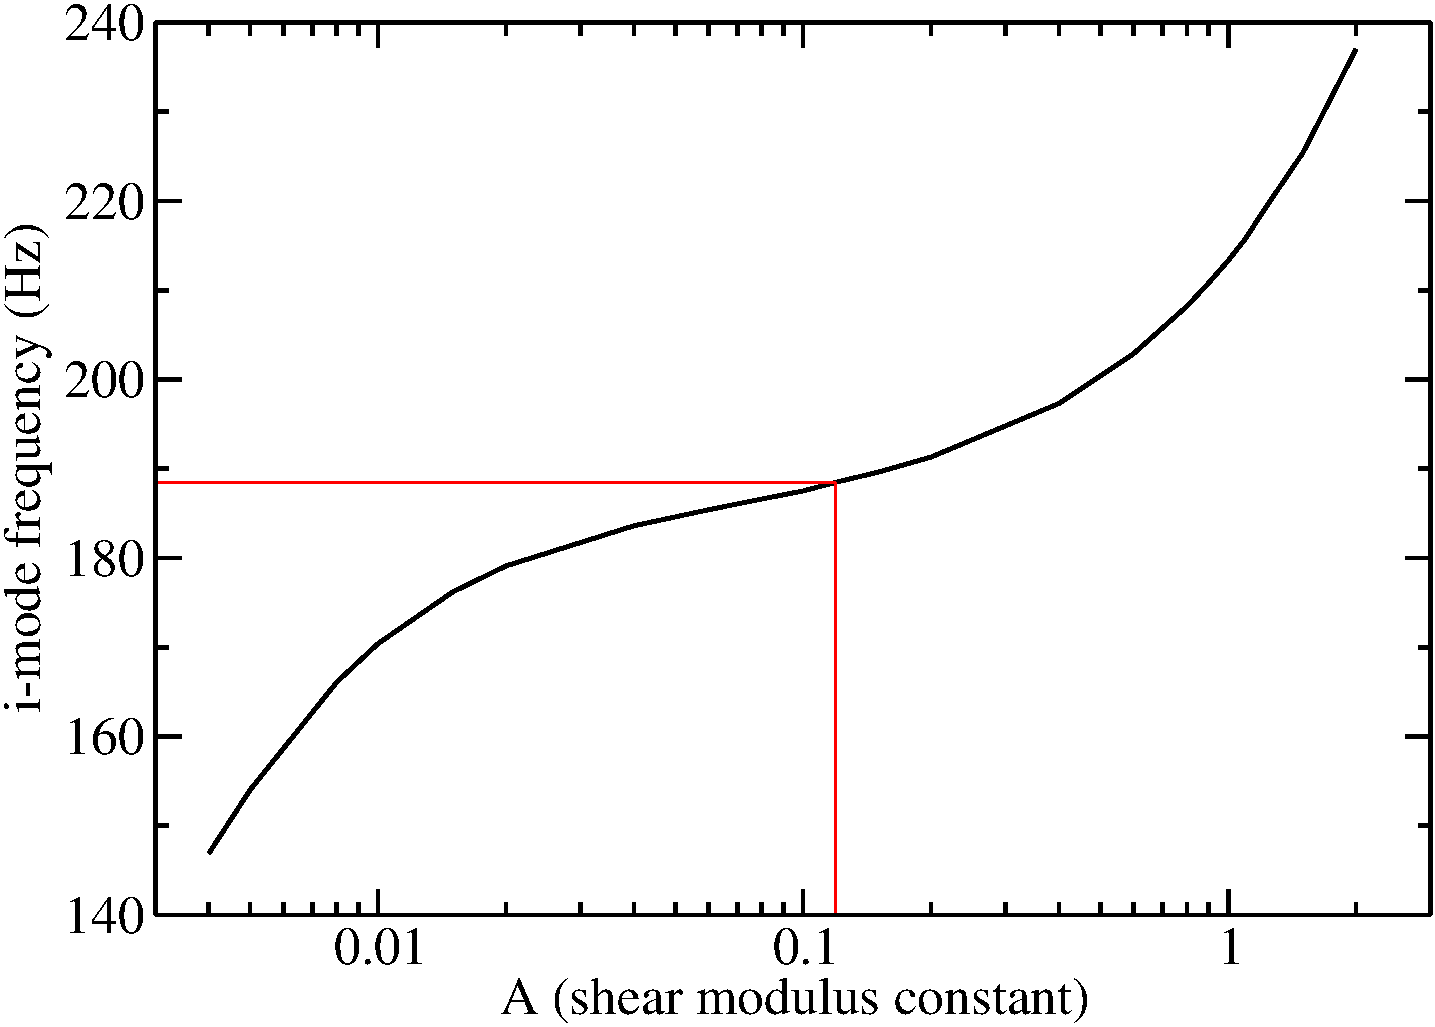
\includegraphics[width=0.45\textwidth,angle=0]{shear_mod_vs_freq}
\caption{The change in i-mode frequency caused by varying $\mu$. The red lines indicate the result for $A=0.1194$.}
\label{fig:mu_A}
\end{figure}










%ALL STARS USED ARE 1.4 SOLAR MASSES

\section{Results}
\hspace{\parindent}Figure \ref{fig:M_vs_f} shows that the mass of the neutron star changes the frequency of the i-mode by up to 20\% from the frequency of a $1.4 M_{\odot}$ star, with the frequency decreasing as the mass of the star is increased.

\begin{figure}
\centering
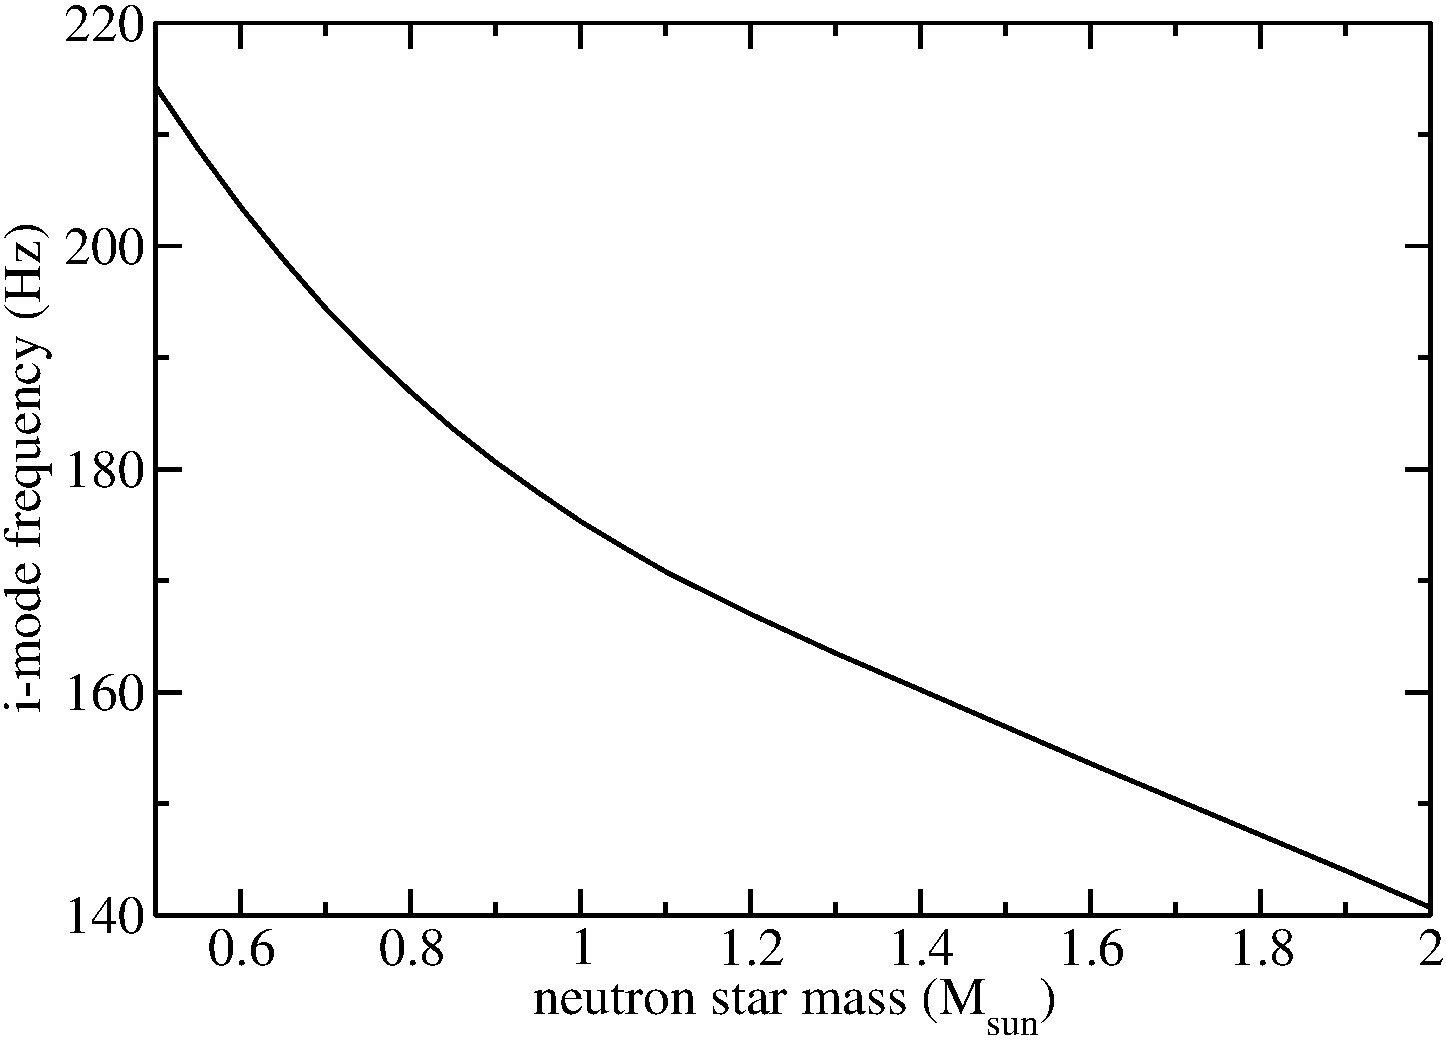
\includegraphics[width=0.45\textwidth,angle=0]{M_vs_f}
\caption{The relationship between NS mass and the i-mode frequency for the sly4 EoS.}
\label{fig:M_vs_f}
\end{figure}






\subsection{Interface Mode dependence on Nuclear Parameters}
\hspace{\parindent}Several EoSs have been generated using a grid of $J$, $L$, and $K_{\rm sym}$ values. By using these EoSs as inputs to find the i-mode frequency for $1.4M_{\odot}$ neutron stars and interpolating between them, we obtained a set of frequency contours in the $J,L$ plane. This is shows in figure \ref{fig:freq_contours}, with the two graphs showing either end of a reasonable $K_{\rm sym}$ range. From this we see that changes in $L$ and $K_{\rm sym}$ have larger impacts on the the i-mode frequency than changes in $J$, as would be expected for a neutron star, in which matter is highly asymmetric.


\begin{figure}
\centering
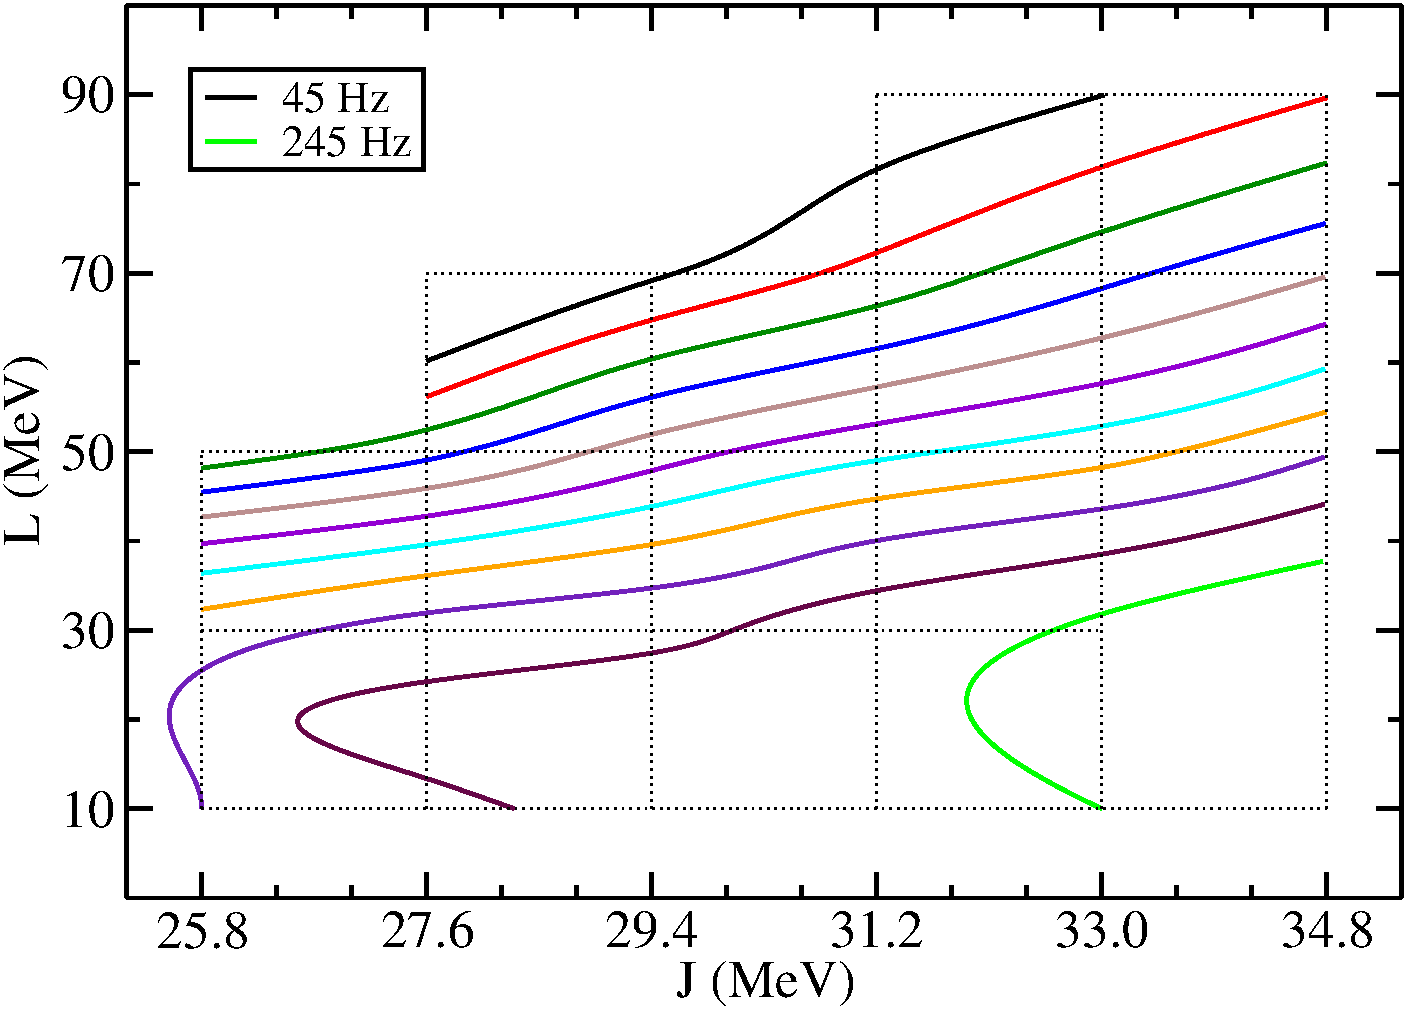
\includegraphics[width=0.45\textwidth,angle=0]{contours_20gap_K40}
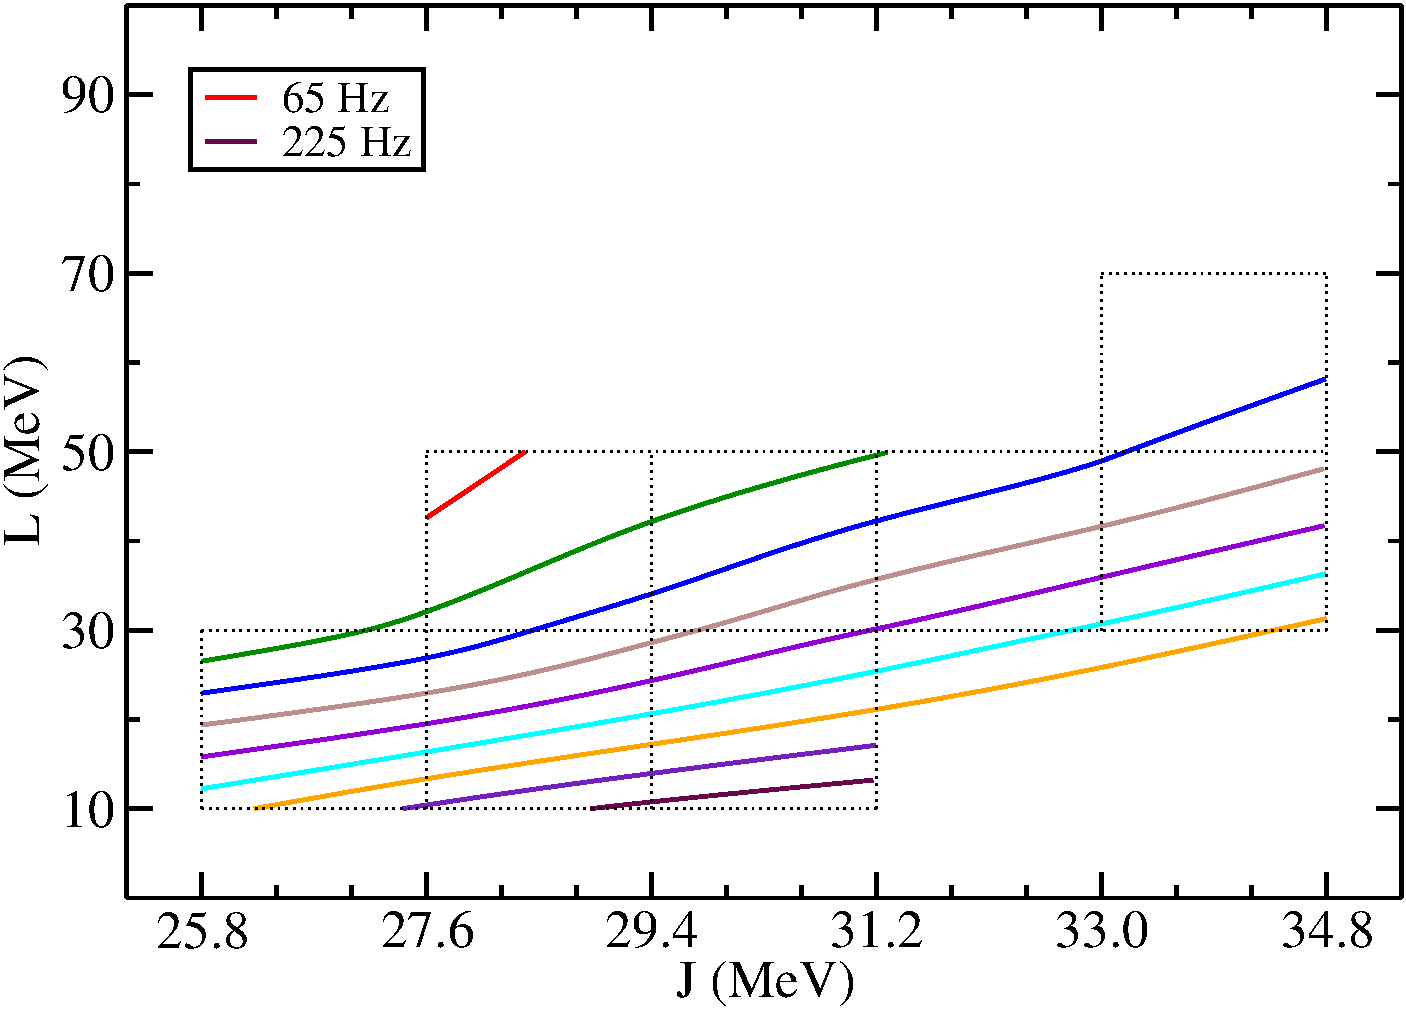
\includegraphics[width=0.45\textwidth,angle=0]{contours_20gap_Km200}
\caption{Frequency contours in the $J,L$ plane, with the first figure being for $K_{\rm sym}=40$ MeV, and the second for $K_{\rm sym}=-200$ MeV. The gaps between the contours are $20$ Hz. The dotted grid indicates the data points that were interpolated between.}
\label{fig:freq_contours}
\end{figure}








\subsection{Constraining $J$, $L$, and $K_{\rm sym}$ with an RSF detection}
\hspace{\parindent}The timescale over which resonant excitation of a mode can occur is calculated as \cite{tsang2012resonant}
\begin{align}
t_{\rm res}\sim 8\times10^{-2}s\left(\frac{\mathcal{M}}{1.2M_{\odot}}\right)^{\frac{-5}{6}}\left(\frac{f_{mode}}{100 \text{ Hz}}\right)^{\frac{-11}{6}},
\label{res_timescale}    
\end{align}
\noindent where $\mathcal{M}=\frac{M_1^{\frac{3}{5}}M_2^{\frac{3}{5}}}{(M_1+M_2)^{\frac{1}{5}}}$ is the chirp mass. From this the resonance window gets smaller as the frequency increases, giving a smaller range over which the resonance will be spread. For a resonance at $100$ Hz and a chirp mass of $1M_{\odot}$, $t_res\sim 0.093$ Hz. This means that the spread of the contour in the $J,L$ is tiny, and so the main uncertainty will come from the value of $K_{\rm sym}$, which causes a spread of up to $\sim 20$ MeV in $L$ at any given $J$ value.




\section{Discussion}
The contours in figure \ref{fig:freq_contours} ...............
%far from symmetry, so we would expect higher order terms (L,Ksym) to have a stronger impact on the frequency than lower order terms (J). This does seem to be the case.




\subsection{Comparisons to other constraints}
\hspace{\parindent}There are many different constraints on the symmetry energy parameters that can be found from various properties of nuclei, such as the their masses %REFERENCE
and neutron skins. %REFERENCE
By plotting these constraints together, a small range can be found for the symmetry energy parameters $J$ and $L$~\cite{balantekin2014nuclear}. This range is shown in figure \ref{fig:constraints} alongside the contours for an supposed detection of a RSF at $100$ Hz, with the two contours showing the range of $K_{\rm sym}$ values. 100 $Hz$ was chosen because the precursor occurs roughly half a second before the merger \cite{zhong2019precursors}, and half a second before the merger, the frequency of GW170817 was $~100-150$ Hz \cite{abbott2017merger}.
% on the graph of constraints in the J,L plane, my results are similar to those for dipole polarisability (the range in my results is the difference between the K=-200 and K=40 contours)
%further constrain K using the J,L values?

\begin{figure}
\centering
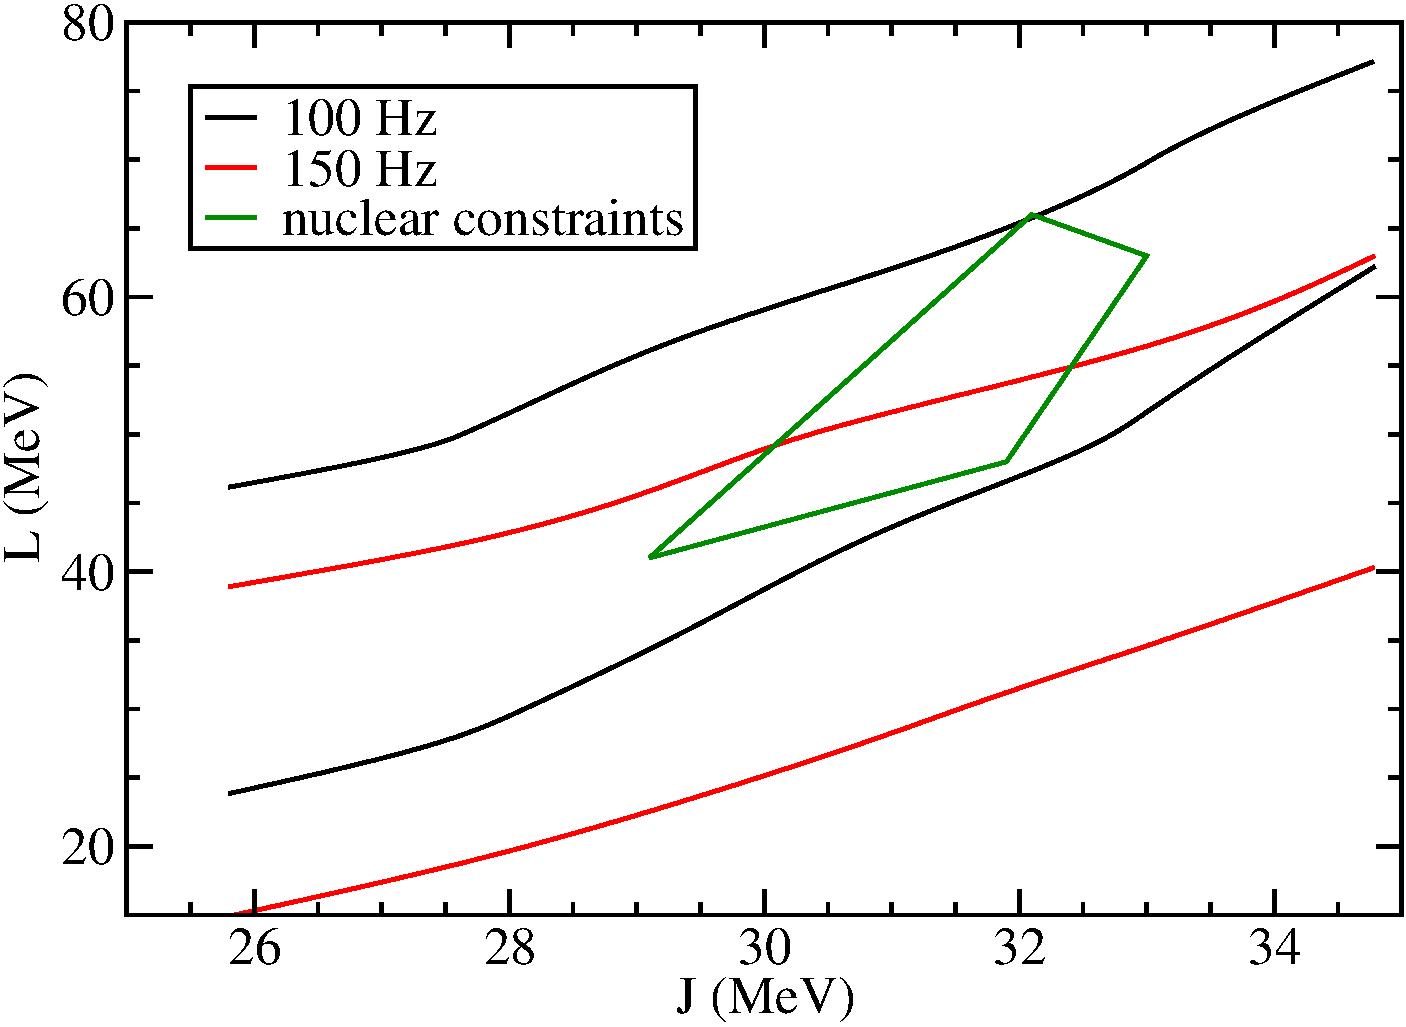
\includegraphics[width=0.45\textwidth,angle=0]{constraints_rough_2}
\caption{<Very rough, replace later>} %Upper bound is K=40 MeV, lower bound is K=-200 MeV.
\label{fig:constraints}
\end{figure}

\hspace{\parindent}From figure \ref{fig:constraints} we see that for an i-mode frequency of $100$ Hz, our constraint applies a similar restriction to the nuclear constraints, making this a useful angle from which to view the restrictions of the values of $J$ and $L$. However, for an i-mode frequency of $150$ Hz, the constraint is shifted to significantly lower L values. Therefor a detection of a precursor at $150$ Hz would improve the previous constraints on $J$ and $L$ to approximately $J\approx 30.75\pm 1.65$ MeV, $L\approx 48\pm 7$ MeV. In general, these results prefer $L$ values towards to lower end of the previous constrains.






%error in mass of binary neutron stars -> range in mass -> get range in i-mode frequencies -> get example error bars in contours.
%2 precursors?

\begin{figure}
\centering
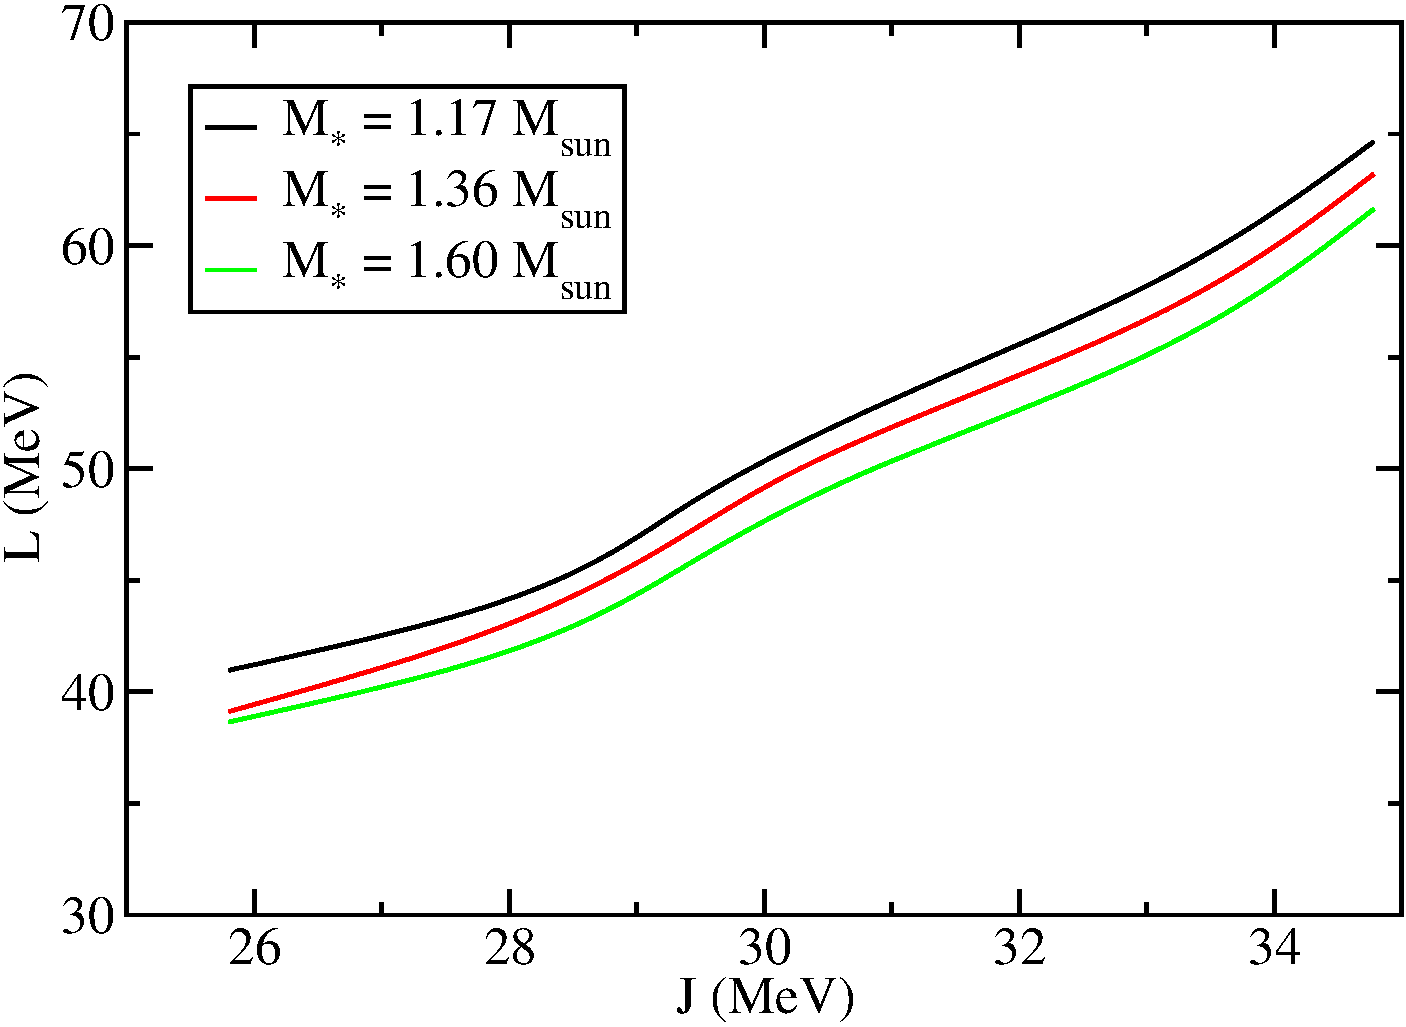
\includegraphics[width=0.45\textwidth,angle=0]{K40_f150_Mcomp.pdf}
\caption{}
\label{fig:vary_mass_contours}
\end{figure}

\begin{figure}
\centering
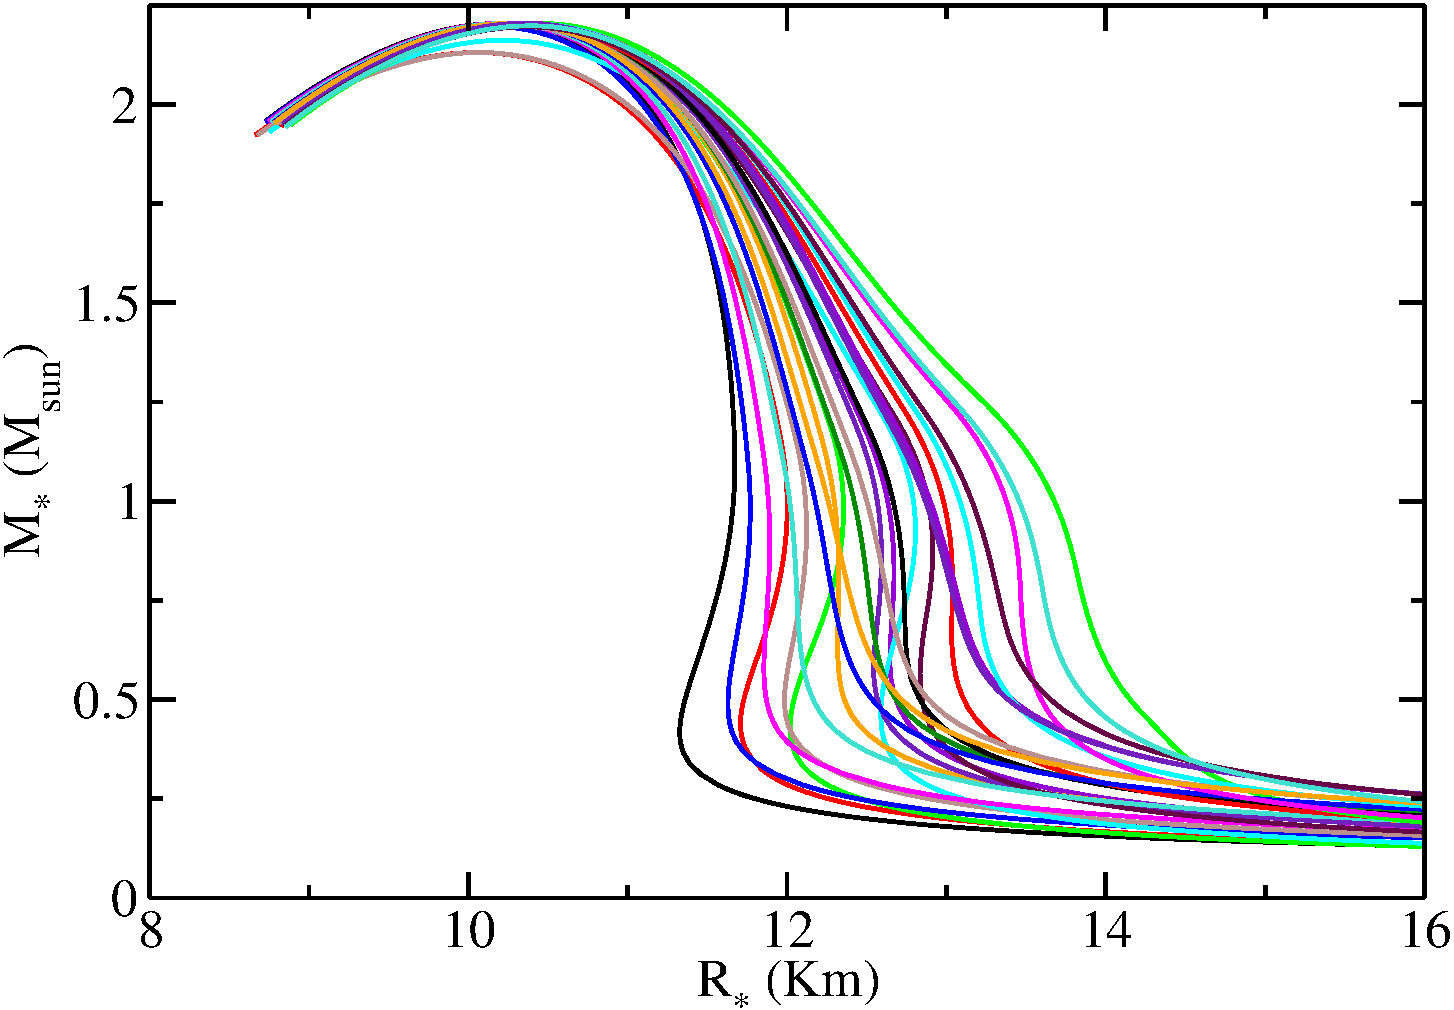
\includegraphics[width=0.45\textwidth,angle=0]{TOVs.pdf}
\caption{}
\label{fig:TOVs}
\end{figure}















%%%%%%%%%%%%%%%%%%%% REFERENCES %%%%%%%%%%%%%%%%%%

% The best way to enter references is to use BibTeX:

\bibliographystyle{mnras}
\bibliography{example} % if your bibtex file is called example.bib


% Alternatively you could enter them by hand, like this:
% This method is tedious and prone to error if you have lots of references
%\begin{thebibliography}{99}
%\bibitem[\protect\citeauthoryear{Author}{2012}]{Author2012}
%Author A.~N., 2013, Journal of Improbable Astronomy, 1, 1
%\bibitem[\protect\citeauthoryear{Others}{2013}]{Others2013}
%Others S., 2012, Journal of Interesting Stuff, 17, 198
%\end{thebibliography}

%%%%%%%%%%%%%%%%%%%%%%%%%%%%%%%%%%%%%%%%%%%%%%%%%%

%%%%%%%%%%%%%%%%% APPENDICES %%%%%%%%%%%%%%%%%%%%%

\appendix

\section{Some extra material}

If you want to present additional material which would interrupt the flow of the main paper,
it can be placed in an Appendix which appears after the list of references.

%%%%%%%%%%%%%%%%%%%%%%%%%%%%%%%%%%%%%%%%%%%%%%%%%%


% Don't change these lines
\bsp	% typesetting comment
\label{lastpage}
\end{document}

% End of mnras_template.tex
